\section{Proposed Method}
\label{sec:method}

\begin{figure*}[t]
  \centering
  % \fbox{\rule{0pt}{2in} \rule{0.9\linewidth}{0pt}}
   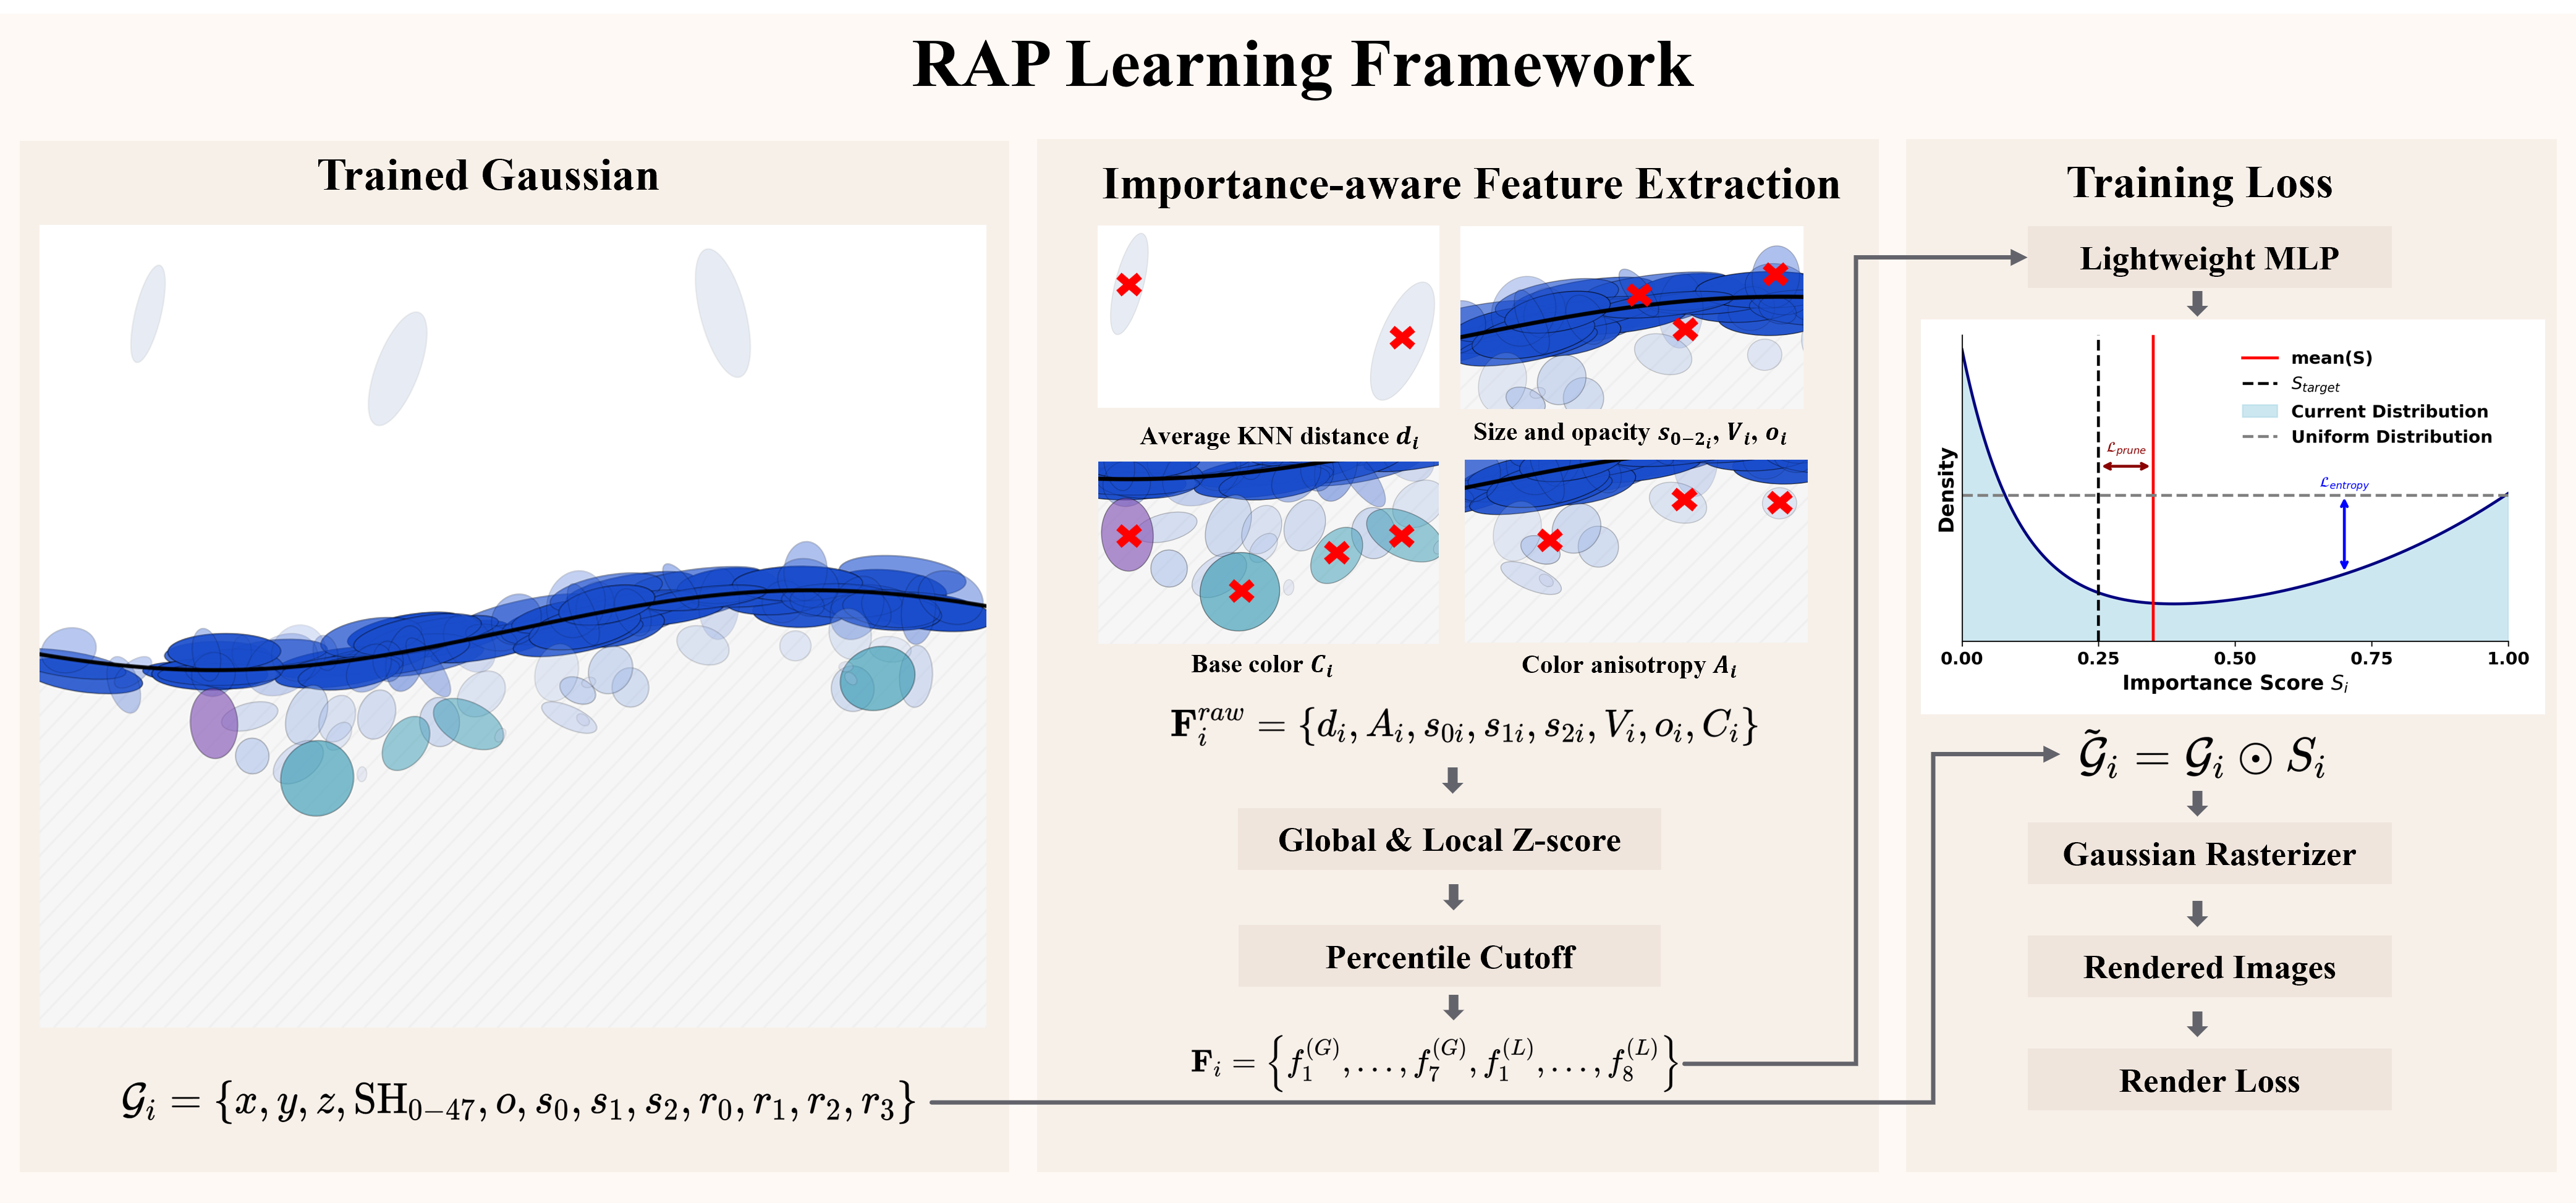
\includegraphics[width=0.9\linewidth]{sec/imgs_main/framework.png}

   \caption{RAP learning framework.}
   \label{fig:framework}
   \vspace{-1.5em}
\end{figure*}

Our proposed RAP framework consists of two stages. First, we perform importance-aware feature extraction, where each Gaussian is represented by a set of importance-related features derived from intrinsic attributes and local neighborhood statistics. These features are then normalized to ensure consistency across different scenes. 
Second, we employ a learning-based importance prediction module, in which a lightweight MLP maps the extracted features to importance scores. Three carefully designed loss functions are proposed to make sure the predicted importance scores are stably distributed from 0 to 1, resulting in flexible, effective, and strong generalization across datasets and downstream GS processing tasks.


\subsection{Importance-aware Feature Extraction}
\label{sec:feature}
We construct a compact 15-dimensional feature vector for each Gaussian primitive by combining intrinsic geometric and appearance attributes with normalized statistics, which consist of three steps: feature computation, feature normalization, and feature concatenation.

$\bullet$\textbf{Feature computation.}
For a Gaussian set $\mathcal{G} = \{\mathcal{G}_1, \ldots, \mathcal{G}_N\}$, each primitive $\mathcal{G}_i$ is represented by a set of raw features,
\begin{equation}
\label{equ:feature}
\mathbf{F}^{raw}_i = \{ d_i, A_i, {s_0}_i, {s_1}_i, {s_2}_i, V_i, o_i, C_i \} \in R^{1\times8},
\end{equation}
where $d_i$ is the average $K$-NN distance, $A_i$ is the color anisotropy, $s_{0,i},s_{1,i},s_{2,i}$ are the sorted Gaussian scales, $V_i$ is the Gaussian volume, $o_i$ is the opacity, and $C_i$ is the DC color. These quantities are computed as follows. 
\begin{itemize}
    \item Average $K$-NN distance:  
    Spatial isolation is measured as
    \begin{equation}
    d_i = \frac{1}{K} \sum_{j \in \mathcal{N}_K(i)} \| \mathbf{p}_i - \mathbf{p}_j \|_2,
    \end{equation}
    where $\mathbf{p}_i \in \mathbb{R}^3$ denotes the spatial position of Gaussian $\mathcal{G}_i$, and $\mathcal{N}_K(i)$ is the set of its $K$ nearest neighbors in Euclidean space.

    \item Color anisotropy:  
    To capture view-dependent appearance variation, we randomly sample $M$ directions $\mathbf{v}_m$ and compute the corresponding RGB colors $\mathbf{c}_i(\mathbf{v}_m)$.  
    The anisotropy is defined as the channel-wise standard deviation across directions:
    \begin{equation}
    A_i = \frac{1}{3} \sum_{c \in \{R,G,B\}} \sigma_m \big( c_i^c(\mathbf{v}_m) \big),
    \end{equation}
    where $\sigma_m$ denotes the standard deviation over sampled directions. A higher $A_i$ indicates a stronger view-dependent color change.
    
    \item Scales and volume:  
    The scales are sorted to ensure rotation invariance:
   $
    s_{0,i} \leq s_{1,i} \leq s_{2,i}.
    $
    The Gaussian volume is then computed as
    \begin{equation}
    V_i = s_{0,i} \times s_{1,i} \times s_{2,i}.
    \end{equation}

    \item Opacity and DC color:  
    Opacity $o_i$ reflects the blending contribution.  
    The DC color $C_i$ is derived from the zeroth-order SH coefficients and averaged over the three RGB channels.
\end{itemize}

$\bullet$\textbf{Feature Normalization.}  
To eliminate scale bias and enhance comparability across Gaussians, each raw feature $f_i \in \mathbf{F}^{raw}_i$ is standardized using both global and local statistics. 
Global normalization $f^{(G)}_i$ applies a scene-wide $z$-score to provide a consistent reference across the entire scene,
% \begin{equation}
% f^{(G)}_i = \frac{f_i - \mu^{(G)}}{\sigma^{(G)}},
% \end{equation}
where $\mu^{(G)}$ and $\sigma^{(G)}$ denote the global mean and standard deviation across all Gaussians. Local normalization $f^{(L)}_i$ further computes a $K$-NN based $z$-score to emphasize local contrast:
\begin{equation}
f^{(G)}_i = \frac{f_i - \mu^{(G)}}{\sigma^{(G)}}, \quad f^{(L)}_i = \frac{f_i - \mu^{(L)}_i}{\sigma^{(L)}_i},
\end{equation}
where $\mu^{(L)}_i$ and $\sigma^{(L)}_i$ are the local mean and standard deviation over the neighbor set $\mathcal{N}_K(i)$. 
For the DC color $C_i$, only local normalization is applied, as color deviation is typically a consequence of local densification while global normalization would be less meaningful due to natural scene characteristics. 

Since z-score normalization centers features around zero with unit variance, the majority of values are expected to fall within $[-3,3]$ according to the empirical three-sigma rule. In practice, however, extreme outliers may still occur. To enhance robustness, all features are clipped to a fixed percentile range and subsequently linearly rescaled to $[0,1]$.

$\bullet$\textbf{Feature Concatenation.}  
Each Gaussian $\mathcal{G}_i$ is ultimately represented as
\begin{equation}
\mathbf{F}_i = \{f^{(G)}_1, \ldots, f^{(G)}_7, f^{(L)}_1, \ldots, f^{(L)}_8\},
\end{equation}
yielding a 15-dimensional vector (7 global + 8 local) that compactly encodes both intrinsic attributes and normalized neighborhood statistics. This representation provides a discriminative yet lightweight basis for importance prediction.


\subsection{Learning Framework and Optimization}
\label{sec:loss}
The features introduced in Sec.~\ref{sec:feature} capture diverse cues correlated with Gaussian primitive importance, but their interactions are highly nonlinear and difficult to model with handcrafted rules. To address this, we employ a lightweight MLP that learns to map the 15-dimensional feature vector $\mathbf{F}_i$ to an importance score. The network takes the normalized feature vector $\mathbf{F}_i$ as input and produces a single-dimensional output, which is passed through a sigmoid activation to yield an importance score $S_i \in [0,1]$. The architecture is intentionally kept lightweight, avoiding convolutions and graph operations, which enables scalability to millions of Gaussians and ensures efficient inference. 

Given a GS scene, we expect the importance scores to be smoothly distributed from 0 to 1. The importance score of each primitive can be explicitly quantified by the influence of pruning this primitive from the scene. Therefore, we adopt three complementary loss functions, ensuring stable and robust predictions by simulating pruning during the training:

$\bullet$\textbf{Rendering Loss.} The first is a rendering loss, which ensures that the rendering quality after pruning based on importance scores is as high as possible. 
For differentiability, each Gaussian’s opacity and scales are softly reweighted by its predicted importance score $S_i$:
\begin{equation}
\tilde{o}_i = o_i S_i, \quad 
\tilde{\mathbf{s}}_i = \mathbf{s}_i S_i, 
\quad \tilde{\mathcal{G}} = \{\tilde{o}_i, \tilde{\mathbf{s}}_i, \text{others}\}.
\end{equation}
The modified set $\tilde{\mathcal{G}}$ is then rendered through the differentiable rasterizer $\mathcal{R}(\cdot)$.
The loss adopts the standard 3DGS formulation:
\begin{align}
\mathcal{L}_{\text{render}} 
&= (1 - \lambda_{\text{dssim}})
   \mathcal{L}_{\text{1}}(\mathcal{R}(\tilde{\mathcal{G}}), I_{\text{gt}}) \nonumber \\
&\quad + \lambda_{\text{dssim}} \,
   \mathcal{L}_{\text{D-SSIM}}(\mathcal{R}(\tilde{\mathcal{G}}), I_{\text{gt}}).
\end{align}
Here, $I_{\text{gt}}$ is the ground-truth reference image. 
This objective encourages the network to suppress redundant primitives while maintaining perceptual consistency with the ground-truth views.

$\bullet$\textbf{Pruning-Aware Loss.} The second loss is a pruning-aware loss, designed to prevent trivial solutions. 
Without additional constraints and only rendering loss, the network could simply assign high importance to all Gaussians. 
To address this, we regularize the mean predicted score by penalizing deviations from a predefined target:
\begin{equation}
\mathcal{L}_{\text{prune}} = \left( \mathrm{mean}(S_i) - S_{\text{target}} \right)^2,
\end{equation}
where $S_{\text{target}}$ specifies a target mean score that explicitly controls the pruning level.
This objective drives the network to suppress redundant primitives in a manner that counterbalances the rendering loss, ensuring that pruning plays a constructive role in model efficiency without sacrificing rendering fidelity.

$\bullet$\textbf{Distribution Regularization.} The third component is a distribution regularization that encourages smooth and diverse importance scores. 
Entropy acts as an intrinsic measure of prediction dispersion; by maximizing entropy, the model avoids collapsing into trivial binary outcomes, thus enabling flexible and adaptive pruning under varying thresholds.
To approximate entropy in a differentiable manner, we construct a soft histogram with $B$ bins using Gaussian kernels, and compute a normalized entropy as
\begin{equation}
\mathrm{EntropyNorm}(S) = 
-\frac{1}{\log B} 
\sum_{k=1}^{B} \tilde{p}_k \log(\tilde{p}_k + \epsilon),
\end{equation}
where $\tilde{p}_k$ denotes the soft bin occupancy. In our case, we expect a larger entropy, the distribution regularization is thus defined as
\begin{equation}
\mathcal{L}_{\text{entropy}} = 1 - \mathrm{EntropyNorm}(S).
\end{equation}
This objective promotes a well-spread distribution of scores within $[0,1]$, enabling pruning thresholds can be flexibly adjusted.

\textbf{Overall Loss.} The overall training objective combines the three components in a weighted sum:
\begin{equation}
\label{eq:loss_total}
\mathcal{L}_{\text{total}} =
\lambda_{\text{render}} \mathcal{L}_{\text{render}} +
\lambda_{\text{prune}} \mathcal{L}_{\text{prune}} +
\lambda_{\text{entropy}} \mathcal{L}_{\text{entropy}}.
\end{equation}
Here, $\lambda_{\text{render}}$, $\lambda_{\text{prune}}$, and $\lambda_{\text{entropy}}$ balance reconstruction fidelity, pruning strength, and score distribution regularization, respectively.

\textbf{Model Training.} 
In each epoch, one view is randomly sampled from one scene to promote generalization across diverse content. 
During training, pruning is simulated in a differentiable manner by softly reweighting Gaussians with their predicted scores, allowing the network to learn how removal influences rendering quality. 
At inference time, no rendering is performed: the normalized feature vector $\mathbf{F}_i$ is fed through the lightweight MLP once to obtain the importance score $S_i$, after which pruning is applied by a fixed threshold or a percentile-based ratio. 
This deployment protocol requires neither scene-specific retraining nor additional rendering, enabling fast, plug-and-play pruning on unseen datasets.
